\documentclass[aspectratio=169]{../latex_main/tntbeamer}  % you can pass all options of the beamer class, e.g., 'handout' or 'aspectratio=43'
\usepackage{dsfont}
\usepackage{bm}
\usepackage[english]{babel}
\usepackage[T1]{fontenc}
%\usepackage[utf8]{inputenc}
\usepackage{graphicx}
\graphicspath{ {./figures/} }
\usepackage{algorithm}
\usepackage[ruled,vlined,algo2e,linesnumbered]{algorithm2e}
\usepackage{hyperref}
\usepackage{booktabs}
\usepackage{mathtools}

\usepackage{amsmath,amssymb}

\DeclareMathOperator*{\argmax}{arg\,max}
\DeclareMathOperator*{\argmin}{arg\,min}

\usepackage{amsbsy}
\newcommand{\vect}[1]{\bm{#1}}
%\newcommand{\vect}[1]{\boldsymbol{#1}}

\usepackage{pgfplots}
\pgfplotsset{compat=1.16}
\usepackage{tikz}
\usetikzlibrary{trees} 
\usetikzlibrary{shapes.geometric}
\usetikzlibrary{positioning,shapes,shadows,arrows,calc,mindmap}
\usetikzlibrary{positioning,fadings,through}
\usetikzlibrary{decorations.pathreplacing}
\usetikzlibrary{intersections}
\pgfdeclarelayer{background}
\pgfdeclarelayer{foreground}
\pgfsetlayers{background,main,foreground}
\tikzstyle{activity}=[rectangle, draw=black, rounded corners, text centered, text width=8em]
\tikzstyle{data}=[rectangle, draw=black, text centered, text width=8em]
\tikzstyle{myarrow}=[->, thick, draw=black]

% Define the layers to draw the diagram
\pgfdeclarelayer{background}
\pgfdeclarelayer{foreground}
\pgfsetlayers{background,main,foreground}

% Requires XeLaTeX or LuaLaTeX
%\usepackage{unicode-math}

\usepackage{fontspec}
%\setsansfont{Arial}
\setsansfont{RotisSansSerifStd}[ 
Path=../latex_main/fonts/,
Extension = .otf,
UprightFont = *-Regular,  % or *-Light
BoldFont = *-ExtraBold,  % or *-Bold
ItalicFont = *-Italic
]
\setmonofont{Cascadia Mono}[
Scale=0.8
]

\renewcommand{\ttdefault}{Cascadia Mono}

% scale factor adapted; mathrm font added (Benjamin Spitschan @TNT, 2021-06-01)
%\setmathfont[Scale=1.05]{Libertinus Math}
%\setmathrm[Scale=1.05]{Libertinus Math}

% other available math fonts are (not exhaustive)
% Latin Modern Math
% XITS Math
% Libertinus Math
% Asana Math
% Fira Math
% TeX Gyre Pagella Math
% TeX Gyre Bonum Math
% TeX Gyre Schola Math
% TeX Gyre Termes Math

% Literature References
\newcommand{\lit}[2]{\href{#2}{\footnotesize\color{black!60}[#1]}}

%%% Beamer Customization
%----------------------------------------------------------------------
% (Don't) Show sections in frame header. Options: 'sections', 'sections light', empty
\setbeamertemplate{headline}{empty}

% Add header logo for normal frames
\setheaderimage{
	% 
\includegraphics[height=\logoheight]{figures/TNT_darkv4.pdf}
	
\includegraphics[height=\logoheight]{../latex_main/figures/Leibniz-AI-Academy_Logo}
	% 
\includegraphics[height=\logoheight]{figures/logo_tntluh.pdf}
}

% Header logo for title page
\settitleheaderimage{
	% 
\includegraphics[height=\logoheight]{figures/TNT_darkv4.pdf}
	
\includegraphics[height=\logoheight]{../latex_main/figures/Leibniz-AI-Academy_Logo}
	% 
\includegraphics[height=\logoheight]{figures/logo_tntluh.pdf}
}

% Title page: tntdefault 
\setbeamertemplate{title page}[tntdefault]  % or luhstyle
% Add optional title image here
%\addtitlepageimagedefault{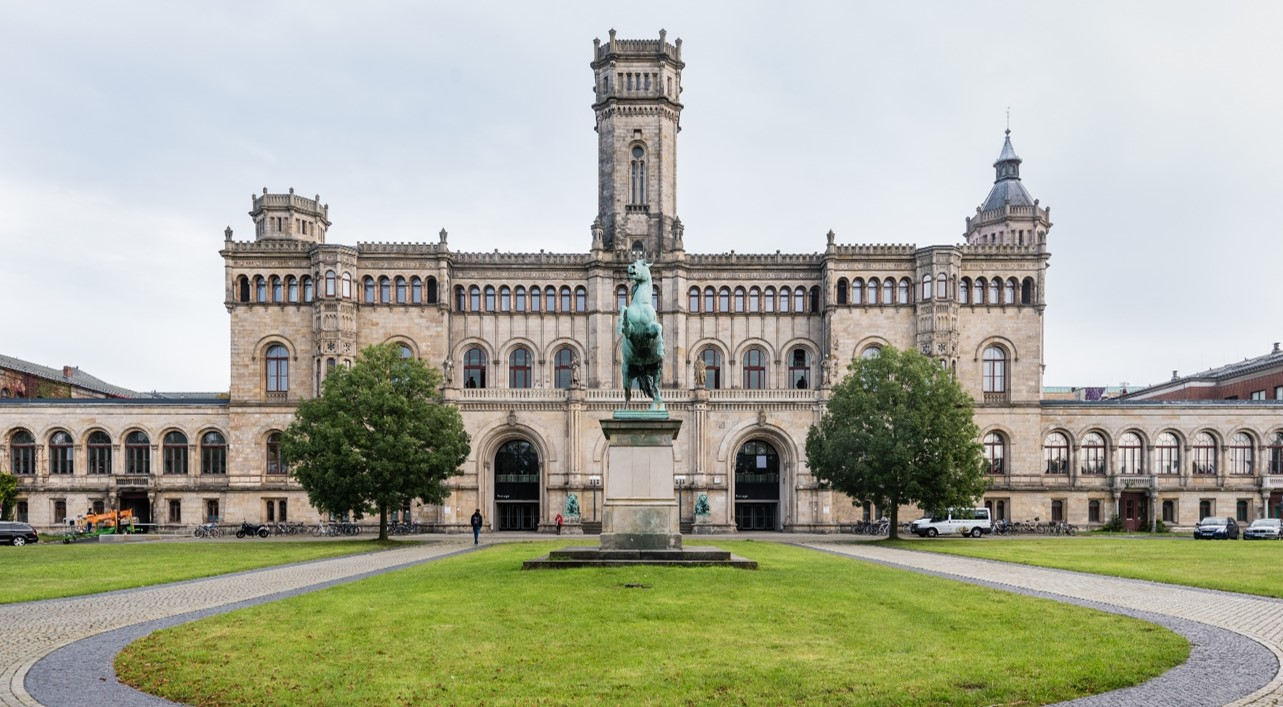
\includegraphics[width=0.65\textwidth]{figures/luh_default_presentation_title_image.jpg}}

% Title page: luhstyle
% \setbeamertemplate{title page}[luhstyle]
% % Add optional title image here
% \addtitlepageimage{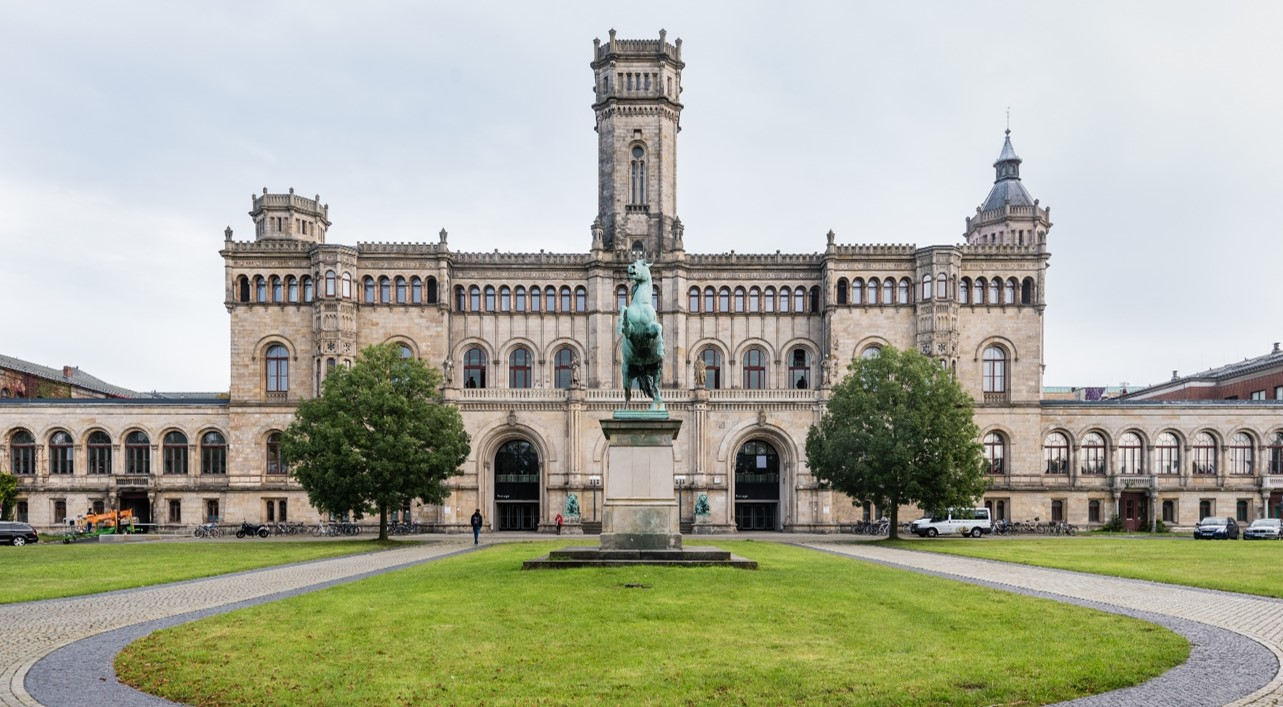
\includegraphics[width=0.75\textwidth]{figures/luh_default_presentation_title_image.jpg}}

\author[Abedjan \& Lindauer]{Ziawasch Abedjan \& \underline{Marius Lindauer}\\[1em]
	%
\includegraphics[height=\logoheight]{../latex_main/figures/luh_logo_rgb_0_80_155.pdf}\qquad
	
\includegraphics[height=\logoheight]{../latex_main/figures/DBIS_Kurzlogo.png}\qquad
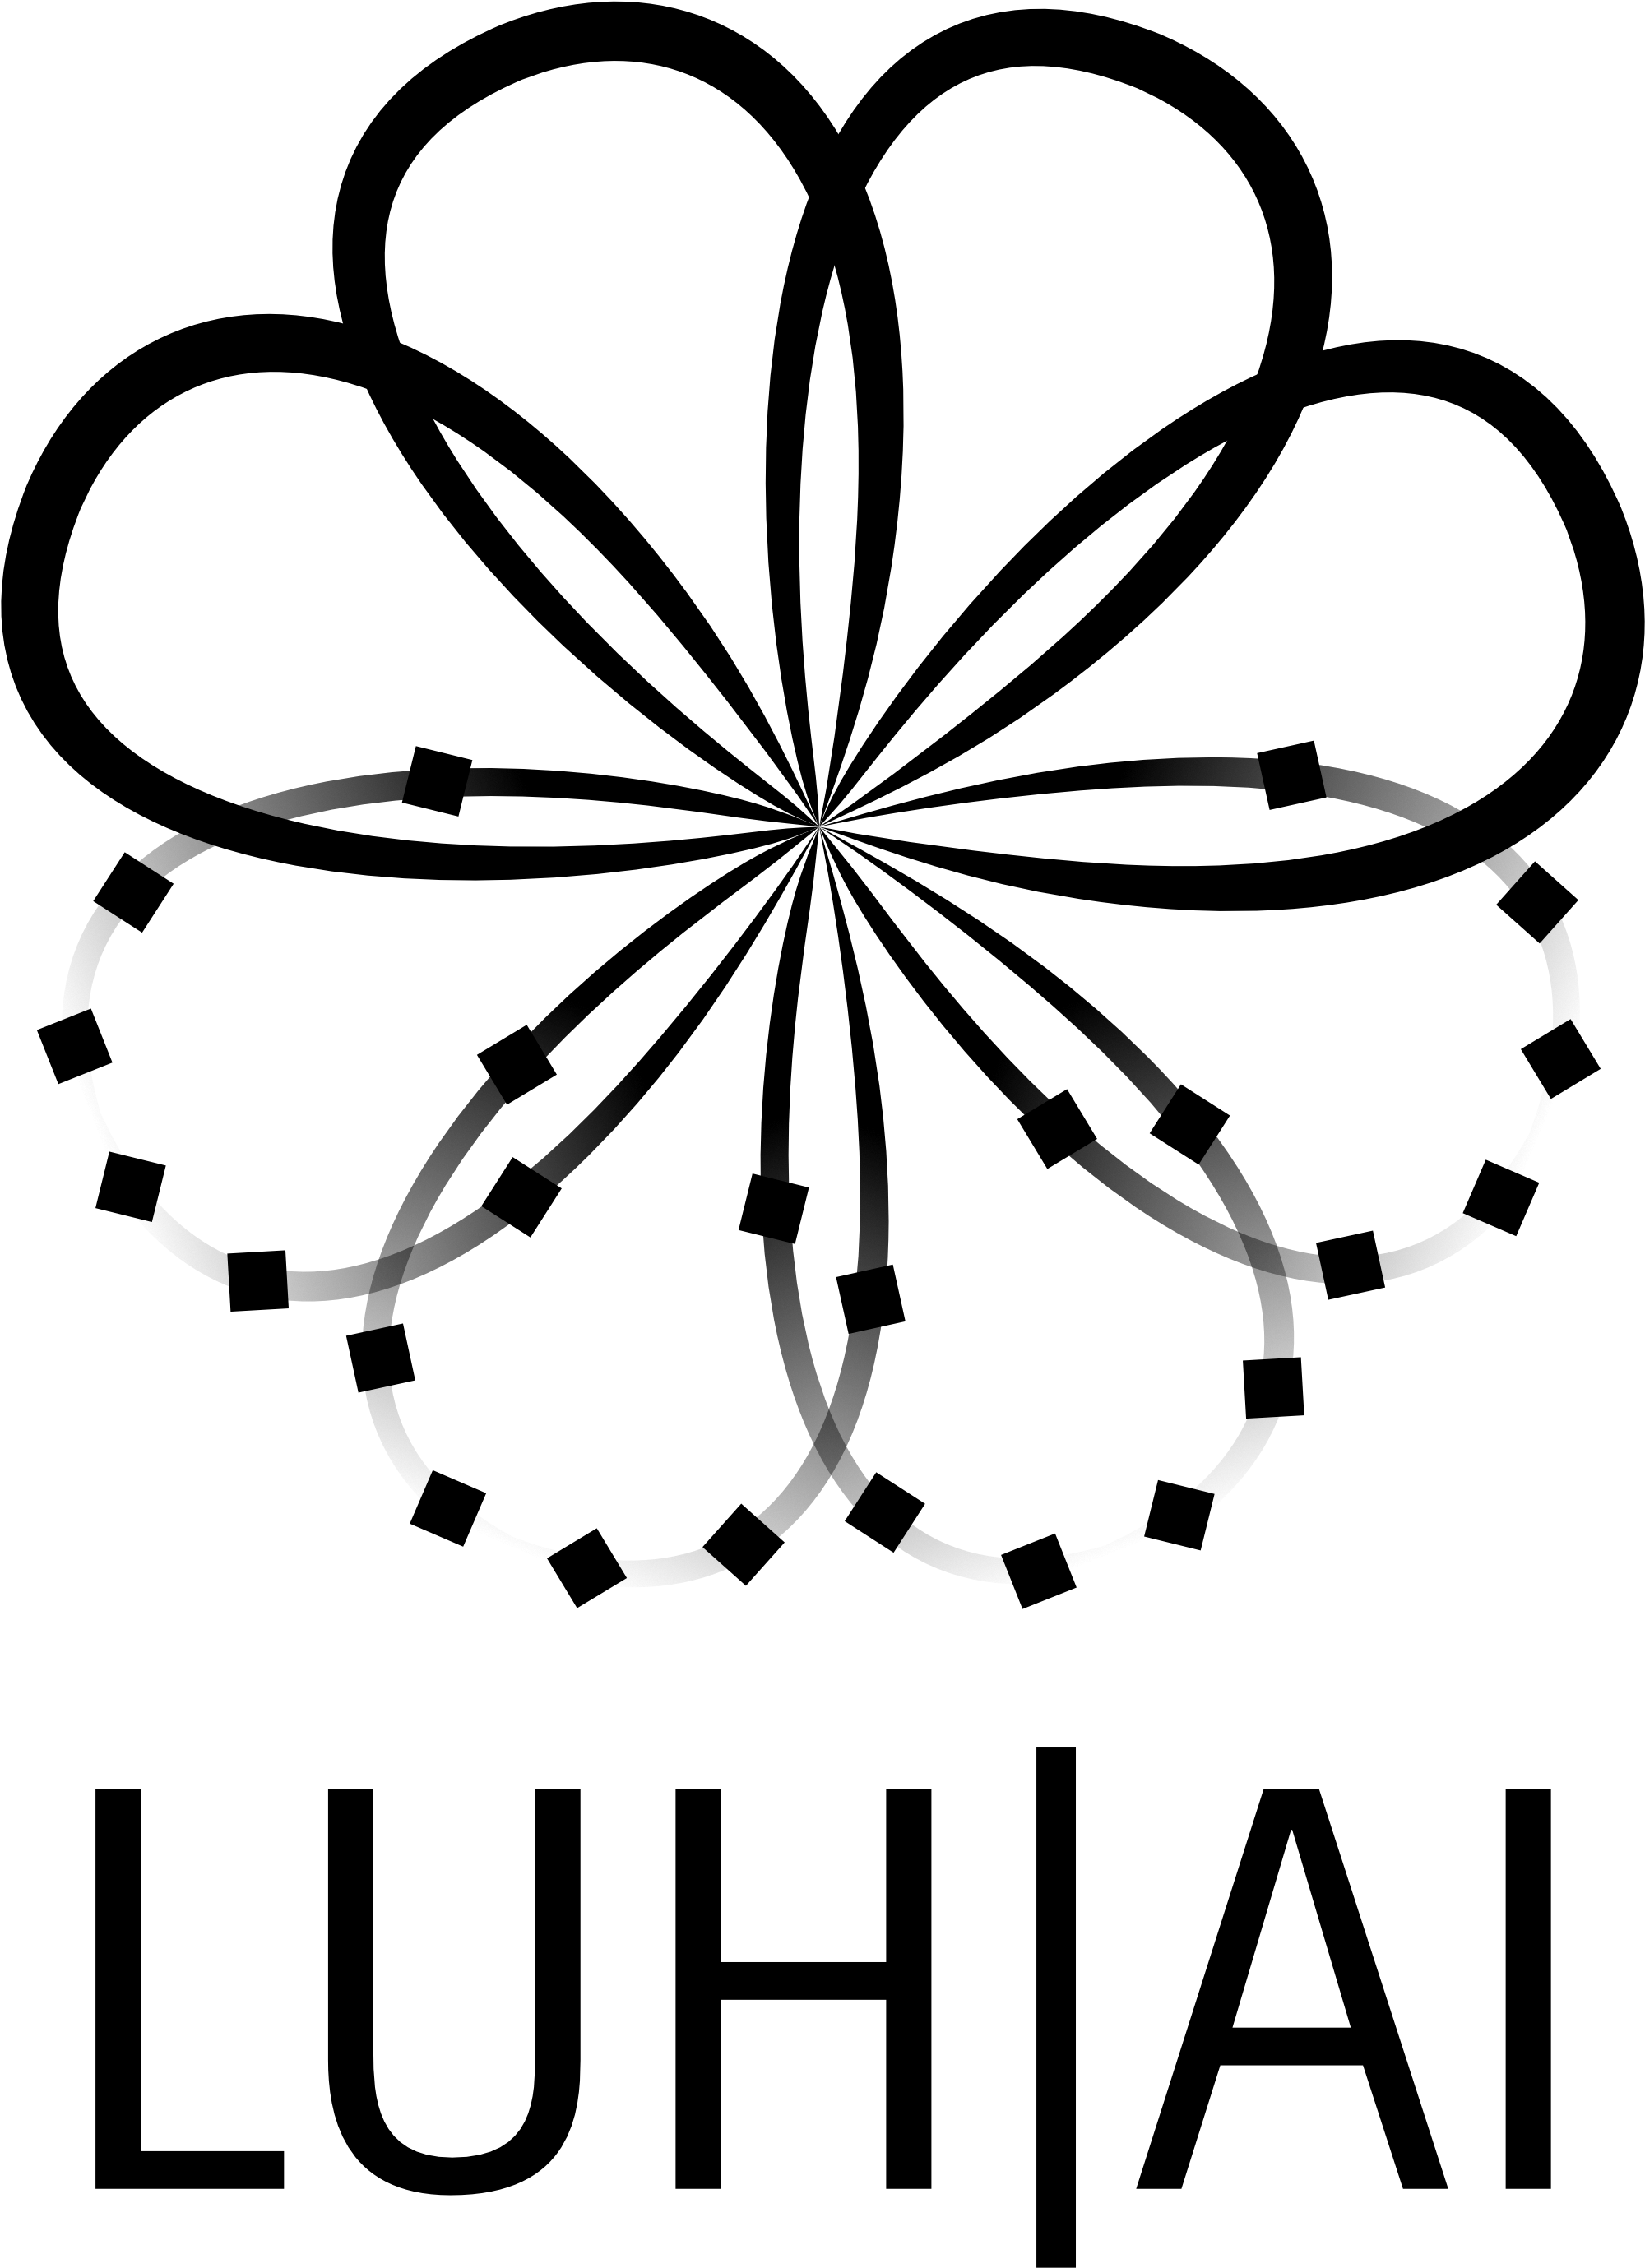
\includegraphics[height=\logoheight]{../latex_main/figures/logo_short_highres_black}\qquad

\includegraphics[height=\logoheight]{../latex_main/figures/Leibniz-AI-Academy_Logo}\qquad
%
\includegraphics[height=\logoheight]{../latex_main/figures/L3S.jpg}	
}
\date{\hspace{0.5em} {
\includegraphics[height=1.5em]{../latex_main/figures/Cc-by-nc-sa_icon.svg.png}}; extension of \href{https://ds100.org/fa21/}{[DS100]}
}


%%% Custom Packages
%----------------------------------------------------------------------
% Create dummy content
\usepackage{blindtext}

% Adds a frame with the current page layout. Just call \layout inside of a frame.
\usepackage{layout}


%%% Macros
%\renewcommand{\vec}[1]{\mathbf{#1}}
% \usepackage{bm}
%\let\vecb\bm

\title[Data Property: Granularity \& Scope]{DS: Data Cleaning}
\subtitle{Data Property: Granularity \& Scope}

\graphicspath{ {./figure/} }
%\institute{}


\begin{document}
	
	\maketitle

\begin{frame}[c]{Key Data Properties to Consider in EDA}
    \begin{itemize}
        \item {Structure} -- the “shape” of a data file.
        \item \textbf{Granularity} -- how fine/coarse is each datum.
        \item {Scope} -- how (in)complete is the data.
        \item {Temporality} -- how is the data situated in time.
        \item {Faithfulness} --how well does the data capture “reality”.
    \end{itemize}
\end{frame}

% Slide 29 - Granularity
\begin{frame}[c]{Granularity}

    \begin{itemize}
        \item What does each record represent?
        \begin{itemize}
            \item Examples: a purchase, a person, a group of users
            \item $\leadsto$ Each of these represents a different level of granularity
        \end{itemize}
        \pause
        \item Do all records capture granularity at the same level?
        \begin{itemize}
            \item Some data will include summaries (aka rollups) as records
            \item $\leadsto$ Pay attention when reasoning over different granularity levels
        \end{itemize}
        \pause
        \item If the data are coarse how was it aggregated?
        \begin{itemize}
            \item Sampling, averaging, …
            \item $\leadsto$ This can be important to know for interpreting the data
        \end{itemize}
    \end{itemize}
\end{frame}

\begin{frame}{Importance of Data Granularity}

\begin{itemize}
    \item {Informs Analysis Precision}
    \begin{itemize}
        \item Determines the level of detail for insights (e.g., daily vs. monthly data).
    \end{itemize}
\pause
    \item {Ensures Relevance and Context}
    \begin{itemize}
        \item Helps align the data's detail level with decision-making needs.
    \end{itemize}
\pause
    \item {Facilitates Data Aggregation and Transformation}
    \begin{itemize}
        \item Allows for effective data summarization and aggregation.
    \end{itemize}
\pause
    \item {Impacts Data Storage and Performance}
    \begin{itemize}
        \item Fine-grained data requires more storage and affects processing speed.
        \item $\leadsto$ Typically, you have more table rows if you consider fine-grained data
    \end{itemize}
\pause
    \item {Improves Data Quality and Consistency}
    \begin{itemize}
        \item Ensures compatibility when merging datasets of different granularity.
    \end{itemize}
\end{itemize}

\end{frame}

\begin{frame}[c]{Key Data Properties to Consider in EDA}
    \begin{itemize}
        \item {Structure} -- the “shape” of a data file.
        \item {Granularity} -- how fine/coarse is each datum.
        \item \textbf{Scope} -- how (in)complete is the data.
        \item {Temporality} -- how is the data situated in time.
        \item {Faithfulness} --how well does the data capture “reality”.
    \end{itemize}
\end{frame}


% Slide 31 - Scope
\begin{frame}[c]{Scope}
    \begin{itemize}
        \item  Does my data cover my area of interest?
        \begin{itemize}
            \item Example: I am interested in studying crime in Hannover but I only have Frankfurt crime data.
        \end{itemize}
        \pause
        \item  Is my data too expansive?
        \begin{itemize}
            \item Example: I am interested in student grades for Data Science Foundations but have student grades for all statistics classes
            \item Solution: Filtering? -- Implications on sample?\\
            $\leadsto$ If the data is a sample I may have poor coverage after filter
        \end{itemize}
        \pause
        \item Does my data cover the right time frame?
        \begin{itemize}
            \item  More on this in temporality...
        \end{itemize}
    \end{itemize}

\end{frame}


% Slide 32 - Sampling Frame
\begin{frame}[c]{Revisiting the Sampling Frame}
    \begin{itemize}
        \item \alert{Reminder:} The sampling frame is the population from which the data was sampled.
        \begin{itemize}
            \item Note that this may not be the population of interest.
        \end{itemize}
        \item How complete/incomplete is the frame (and its data)?
        \item How is the frame/data situated in place?
        \item How well does the frame/data capture reality?
        \item How is the frame/data situated in time?
    \end{itemize}
\end{frame}



\end{document}